% \documentclass[a4paper]{beamer}

\usepackage[english]{babel}
\usepackage[utf8x]{inputenc}
\usepackage{beamerthemesplit}
\usetheme{Berkeley}
\usecolortheme{dolphin}
\usepackage{graphicx}

\mode<presentation>
\author[Surya]{Surya Gaddipati \\ \texttt{sgaddipati@groupon.com}}

\begin{document}
\makeatletter
 \def\beamer@framenotesbegin{% at beginning of slide
   \gdef\beamer@noteitems{}%
   \gdef\beamer@notes{{}}% used to be totally empty.
 }
 \makeatother


\begin{frame}
\titlepage
\frametitle{Perspective Correction}
\framesubtitle{An example application of Linear Algebra}
\end{frame}

\begin{frame}
\frametitle{Objective}
\tableofcontents

\section{A brief introduction to Linear Algebra}
\section{A Motivating example. }
Perspective Correction.
\footnote{Coding The Matrix, https://class.coursera.org/matrix-001/lecture/index (Week 4)}
\end{frame}


\begin{frame}
\frametitle{Vector Spaces}
\begin{center}
\begin{block}{What is a Vector}
\note<1-2>[item]{Moving something from one location to another}
\begin{figure}[ht!]
\centering
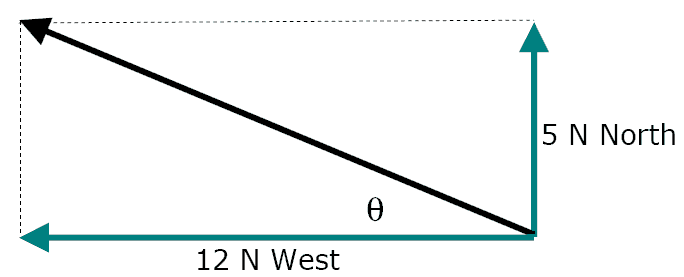
\includegraphics[width=90mm]{vector-example.png}
\caption{A Geometric Representation}
\label{overflow}
\end{figure}

\end{block}
\end{center}
\end{frame}


\end{document}



